
\chapter{Experiment: Speedy bandits} \label{ch:experiment}
Now we return to the question of the exploration-exploitation dilemma. As we have seen, optimal decision strategies are not always available; they require an infinite horizon if the reward distributions are unknown or are computationally too expensive. 

Heuristics like the UCB and the Thompson sampling have successfully been applied to the behavior of participants in experiments where a bandit task was used. Heuristics are, in our case, exploration strategies, these are updated with the help of learning models like the Kalman filter or the BMT. There are two major families of exploration strategies, random exploration and directed exploration, with the Thompson sampling representing the random exploration and the UCB directed exploration. 
Since both, the UCB and the Thompson sampling not include any prediction about reaction time, we applied time pressure on a four armed bandit to gain more insights in how humans choose or use an exploration strategy. 
By inducing time pressure, we reduce the available time to consider a decision. If directed exploration is a reasoned and controlled process, then limited time might influence the balance between directed and random exploration. This will give us a better understanding about how humans use different exploration strategies on a process level. 

We assume that, under time pressure we will find a negative effect on the exploration bonus in directed exploration. Hence, we assume that participants will explore less under time pressure and also avoid risky options. 
%What is the main message you want to convey in this opening section? Why are we running this experiment? What is the main manipulation we are running? What are our hypotheses?

\section{Methods}
\subsection{Participants and design}
We recruited 99 participants (36 female; $M_{age}=34.82$; $SD=10.1$; range: 21 to 69) through Amazon Mechanical Turk (requiring $95\%$ approval rate and $100$ previously approved HITs). A base fee of $\$3.00$ was paid for participation, with a performance contingent bonus of up to $\$4.00$ . On average, participant spent $13.0 \pm$ $5.6$ minutes on the task and earned a total of $\$5.87$ $\pm$ $\$0.97$.  

We used a 2x4 within-subject design, combining either limited or unlimited choice time with four different payoff conditions.
The online-experiment consisted of 40 rounds with 20 trials each. All conditions were conducted in a pseudo-randomized order such that each payoff condition was paired with each time condition five times.

The four armed bandit problem was designed in such a way that the four arms were represented by the Q,W,O and P keys on the keyboard. These keys were randomized for each round. By pressing one of those key on the keyboard participants choose the according arm. 
Participants were informed if the next round was a limited or an unlimited time round. In limited time rounds, participants were given a 400 milliseconds (ms) time window to make each choice. After making a choice under the limit, a smiley icon and the reward value were presented for 400 ms before continuing to the next trial. If participants did not respond within the 400 ms limit, the screen flashed red to indicate time ran out. Participants were still able to choose an option, but the reward was forfeit and a sad smiley appeared with a crossed out reward appeared, also for 400 ms before continuing to the next trial. In unlimited time rounds, participants were always shown the smiley face and reward value, no matter how long they took to make their choice. As in limited time rounds, the feedback lasted 400 ms before continuing to the next trial.

\begin{figure}
    \centering
    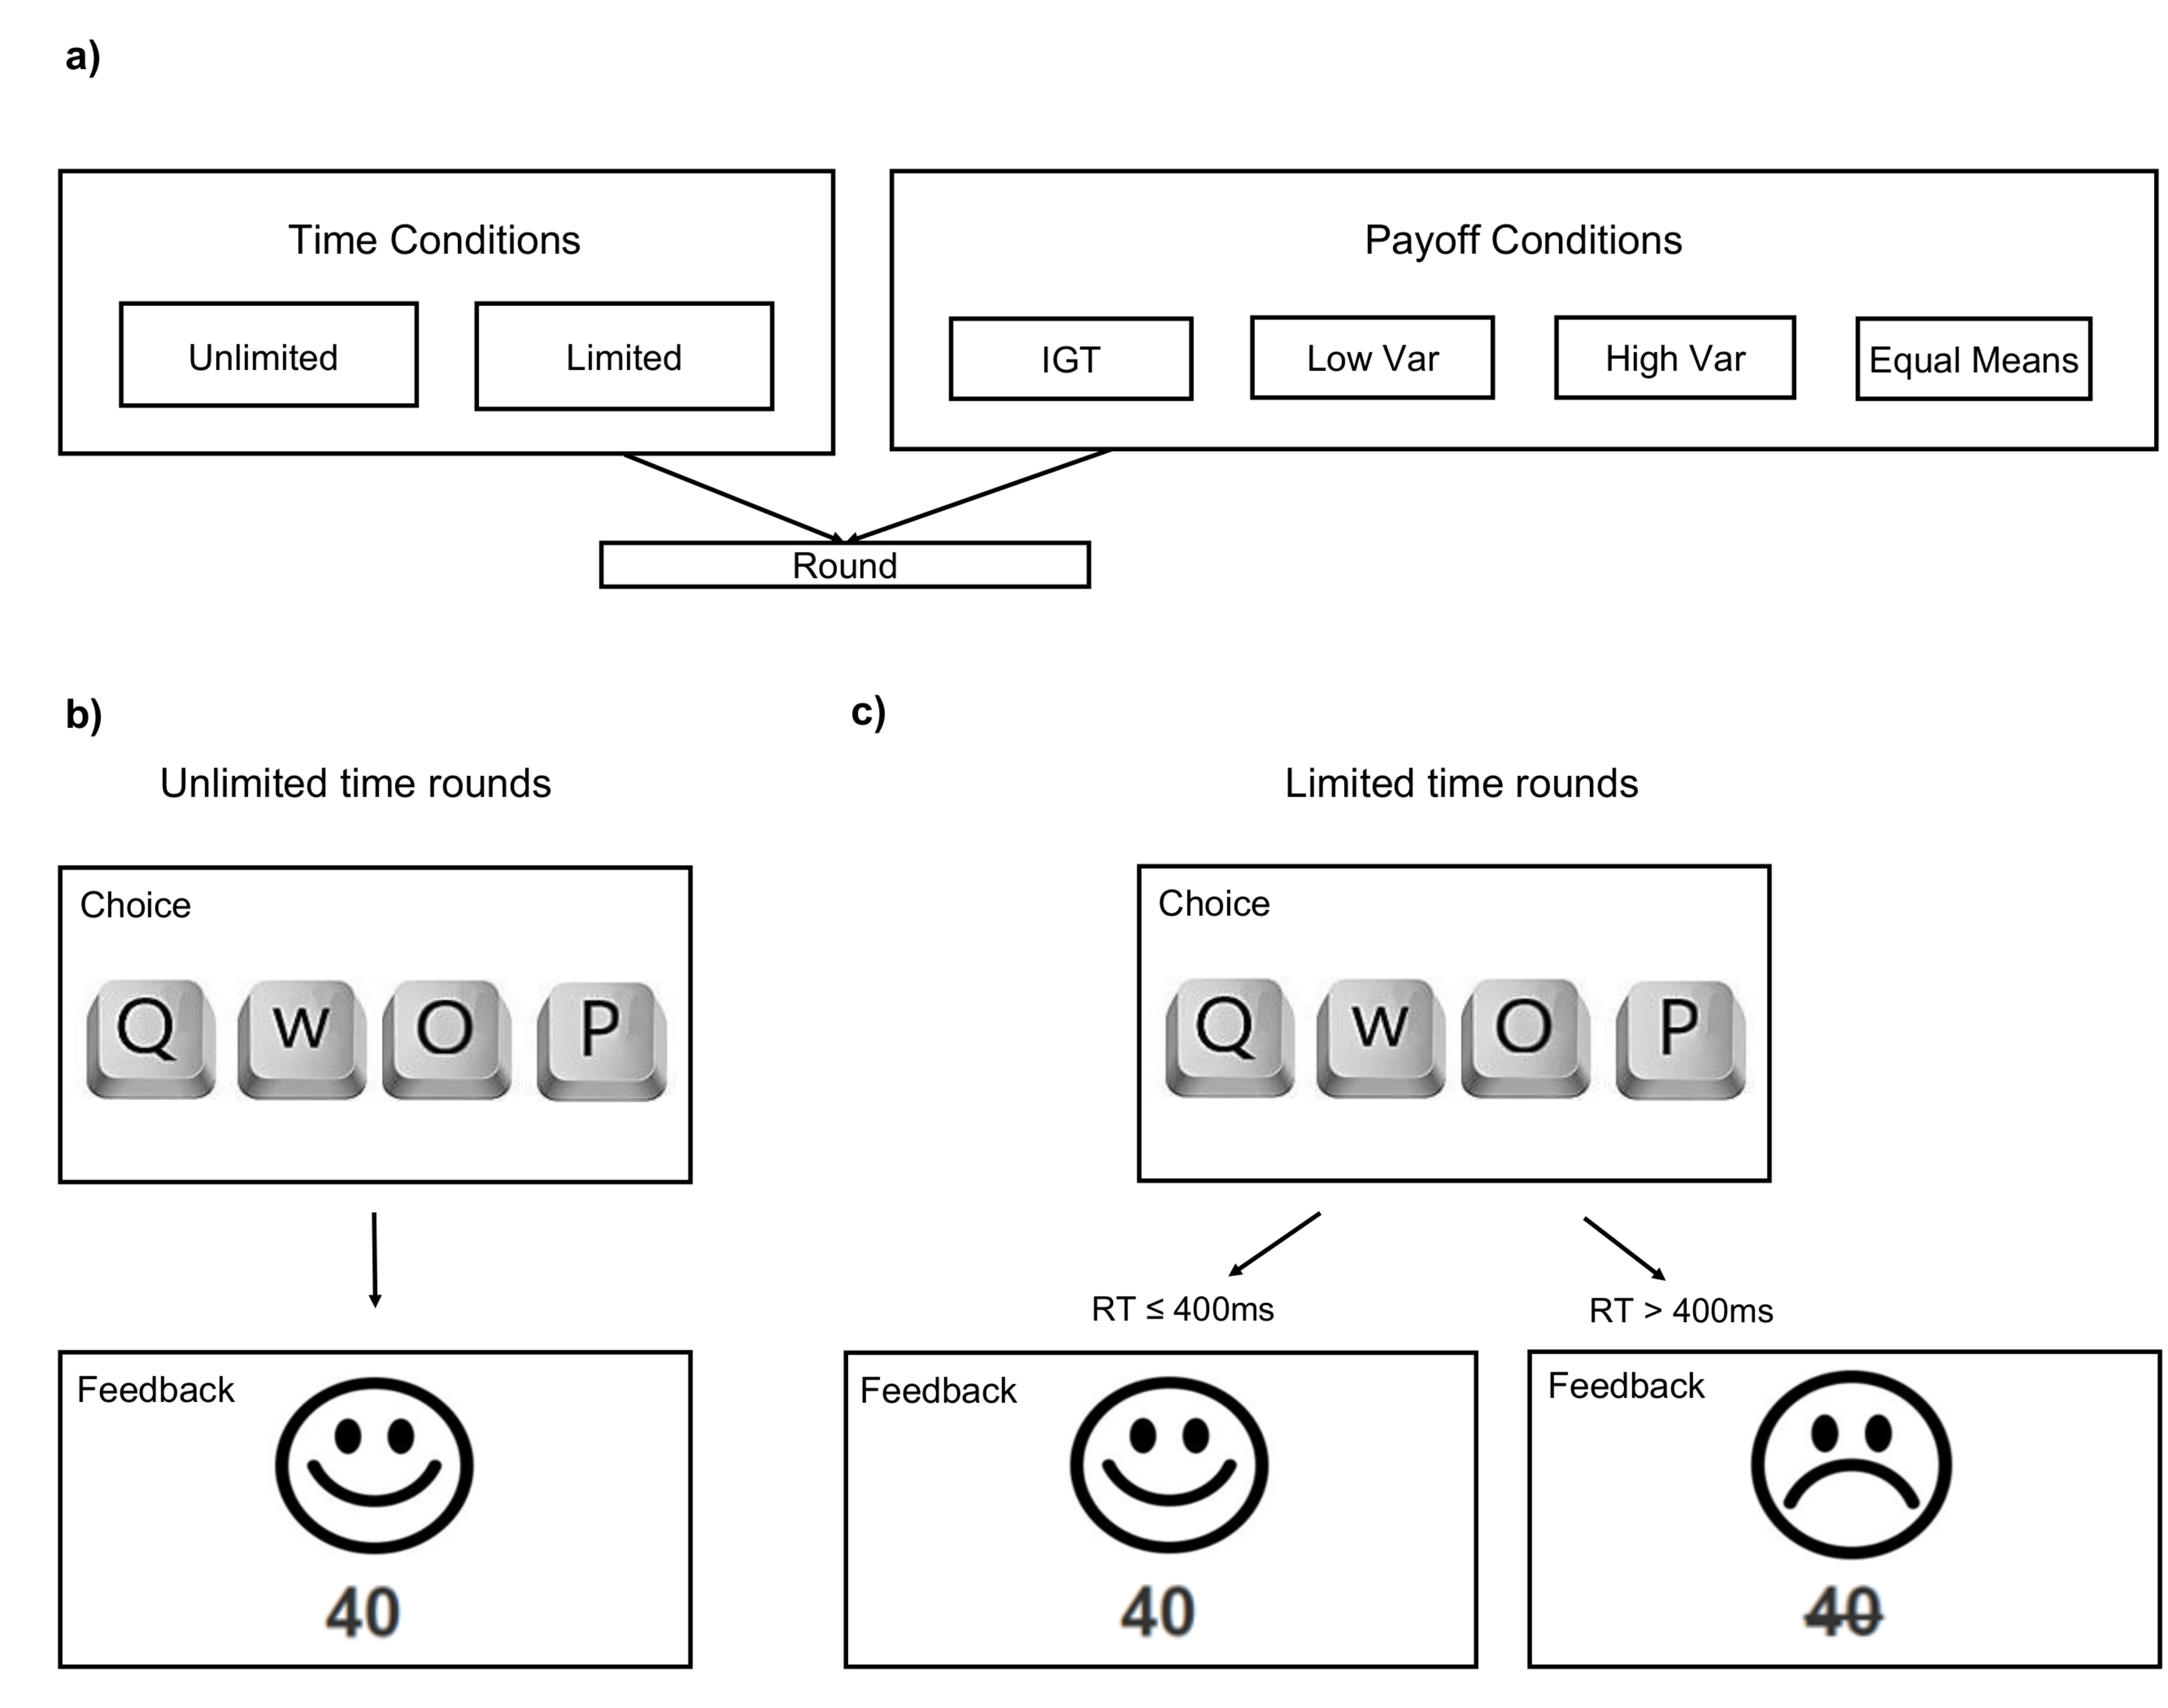
\includegraphics[width=0.8\textwidth]{Plots/ExperimentalSetup.pdf}
    \caption[Experimental Design]{Experimental design. \textbf{a)} Time conditions and payoff conditions were paired in order to form a round. The pairing results in eight different rounds, each was played five times. Participants were informed which time condition they would be in but had no information about the payoff condition. \textbf{b}) In unlimited time rounds, participants were able to choose between four keys, when they pressed the key, a happy smiley appeared with the reward for that trial.  \textbf{c}) In unlimited time rounds, participants had a time window of 400ms to make a choice, if they failed a sad smiley with a crossed out reward appeared to indicated that they did not receive any reward, but still have the information what the reward for this arm could have been. If the participants stayed within the 400ms window, a happy smiley with the reward appeared. }
    \label{fig:Experiment}
\end{figure}


\begin{table}
\vspace{-2mm}
\caption{Payoff Conditions} 
\label{tab:payoffs} 
\begin{tabular*}{\textwidth}{@{}l@{\extracolsep{\fill}}cc@{}}
\toprule
Payoff Conds & Means ($\mu$) & Variances ($\sigma^2$)  \\ \midrule
IGT & $\{-10,-10,10,10\}$ & $\{10,100,10,100\}$      \\
Low Var   & $\{-10,-1/3,1/3,10\}$ & $\{10,10,10,10\}$       \\
High Var & $\{-10,-1/3,1/3,10\}$ & $\{100,100,100,100\}$       \\
Equal Means  & $\{0,0,0,0\}$     & $\{10,40,70,100\}$      \\
\bottomrule
\end{tabular*}
\vspace{5mm}
\end{table}

%Motivate the choice of different payoff conditions as being used to disentangle differences in relative reward vs. relative uncertainty
Payoff conditions determine the mean and the variance of the normally distributed payoff function for each each option (see Fig. \ref{fig:RDistribution}). They were modelled such that absolute and relative uncertainty governed one payoff condition. Relative uncertainty deals with the uncertainty between options, whereas absolute uncertainty is about the overall uncertainty of all options.  
The first payoff condition was inspired by the \emph{Iowa Gambling Task} (IGT), such that there are two high and two low means $\mu_i\in \{-10, -10, 10, 10\}$, as well as two high and two low variance $\sigma^2_i\in \{10, 100, 10, 100\}$. 
We also included \emph{high variance} and \emph{low variance} conditions, where options had equally spaced means $\mu_i \in \{-10, -1/3, 1/3, 10\}$, but where the variances were uniformly low ($\sigma^2=10$) or high ($\sigma^2=100$), respectively. Lastly, we included an \emph{equal means} condition, which had the same mean for all four options ($\mu=0$) but with equally spaced variances $\sigma^2_i\in \{10,40, 70, 100\}$). 
Each reward was presented with a symbol (e.g., $\rho, \phi, \vartheta$ ) which indicates a foreign currency, so it is not clear how much the reward would translate to USD. To strengthen this intuition, rewards were shifted by adding a number sampled from a uniform distribution $U(30, 60)$ for each round. This shifted the normal distribution in a way that negative rewards were unlikely, if however a negative reward was still sampled, it was sampled again.  
It is clear however, that the higher the reward the better the real world outcome. 


\begin{figure}
    \centering
    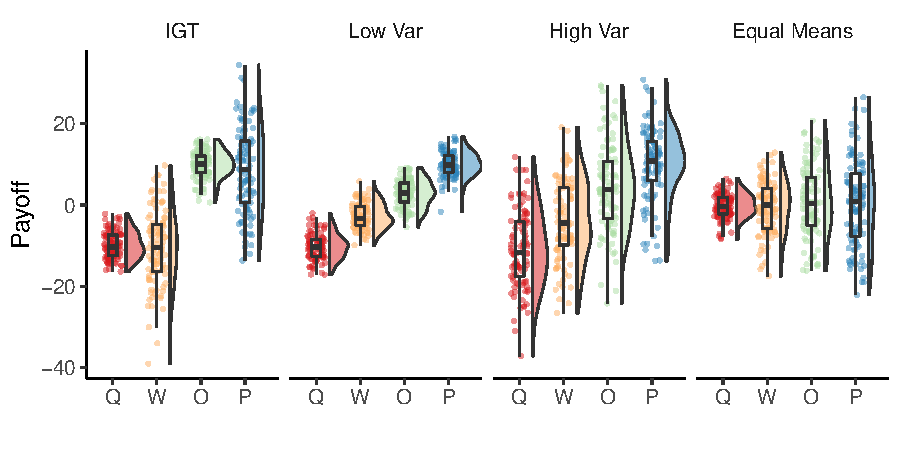
\includegraphics{Plots/RewardDistributions2.pdf}
    \caption[Reward Distributions]{Reward Distributions. These are 100 samples for each of the distribution in each payoff condition. Those are not the actual rewards participants saw, since those were shifted with a uniform distribution.}
    \label{fig:RDistribution}
\end{figure}



\subsection{Materials and Procedure}
After the instructions, participants where asked to answer three comprehension questions in order to ensure they understood the task. After successfully answering the comprehension questions, participants completed a practice round with five trials for each time condition, in order to gain familiarization with the limited and unlimited time conditions.  

To start each new round, participants were informed whether it was a limited or unlimited time round, and were instructed to put their fingers on the Q,W,O, and P keys before pressing the spacebar to continue.
Participants were paid a bonus by randomly selecting the performance of one round. They knew in the beginning that each round could be picked, this ensured that they paid attention in each round. 
After each round, participants were informed about their performance and saw the real monetary bonus they would gain for the round, if this round was the selected round for the bonus.
The performance contingent bonus was calculated as a percentage of the total possible performance, raised to the power of 4 to accentuate differences in the upper range of performance:$$\textup{Bonus} = \left(\frac{\textup{total reward gained}}{\textup{mean reward of best option} \times 20 \textup{ trials}}\right)^4 \times \$4.00$$
Participants were informed that one round would be randomly selected as the basis for their bonus. 

\section{Behavioral Results}
\subsection{Learning Curves}
Participants were able to learn to perform better over trials in all but the Equal Means condition, because the means did not change and thus a better option is not available. Participants learned the fastest in the IGT condition, followed by the Low Variance condition and the High Variance condition. Trials and performance are correlated (average correlation: Spearman's $\rho =  0.16$, $t(98)=21.8$, $p< .001$, $BF > 100$). 
However, there was no difference in correlation between limited and unlimited time rounds ($t(98)=-1.3, p=.96, d=0.13, BF=0.25$).
\begin{figure}
    \centering
    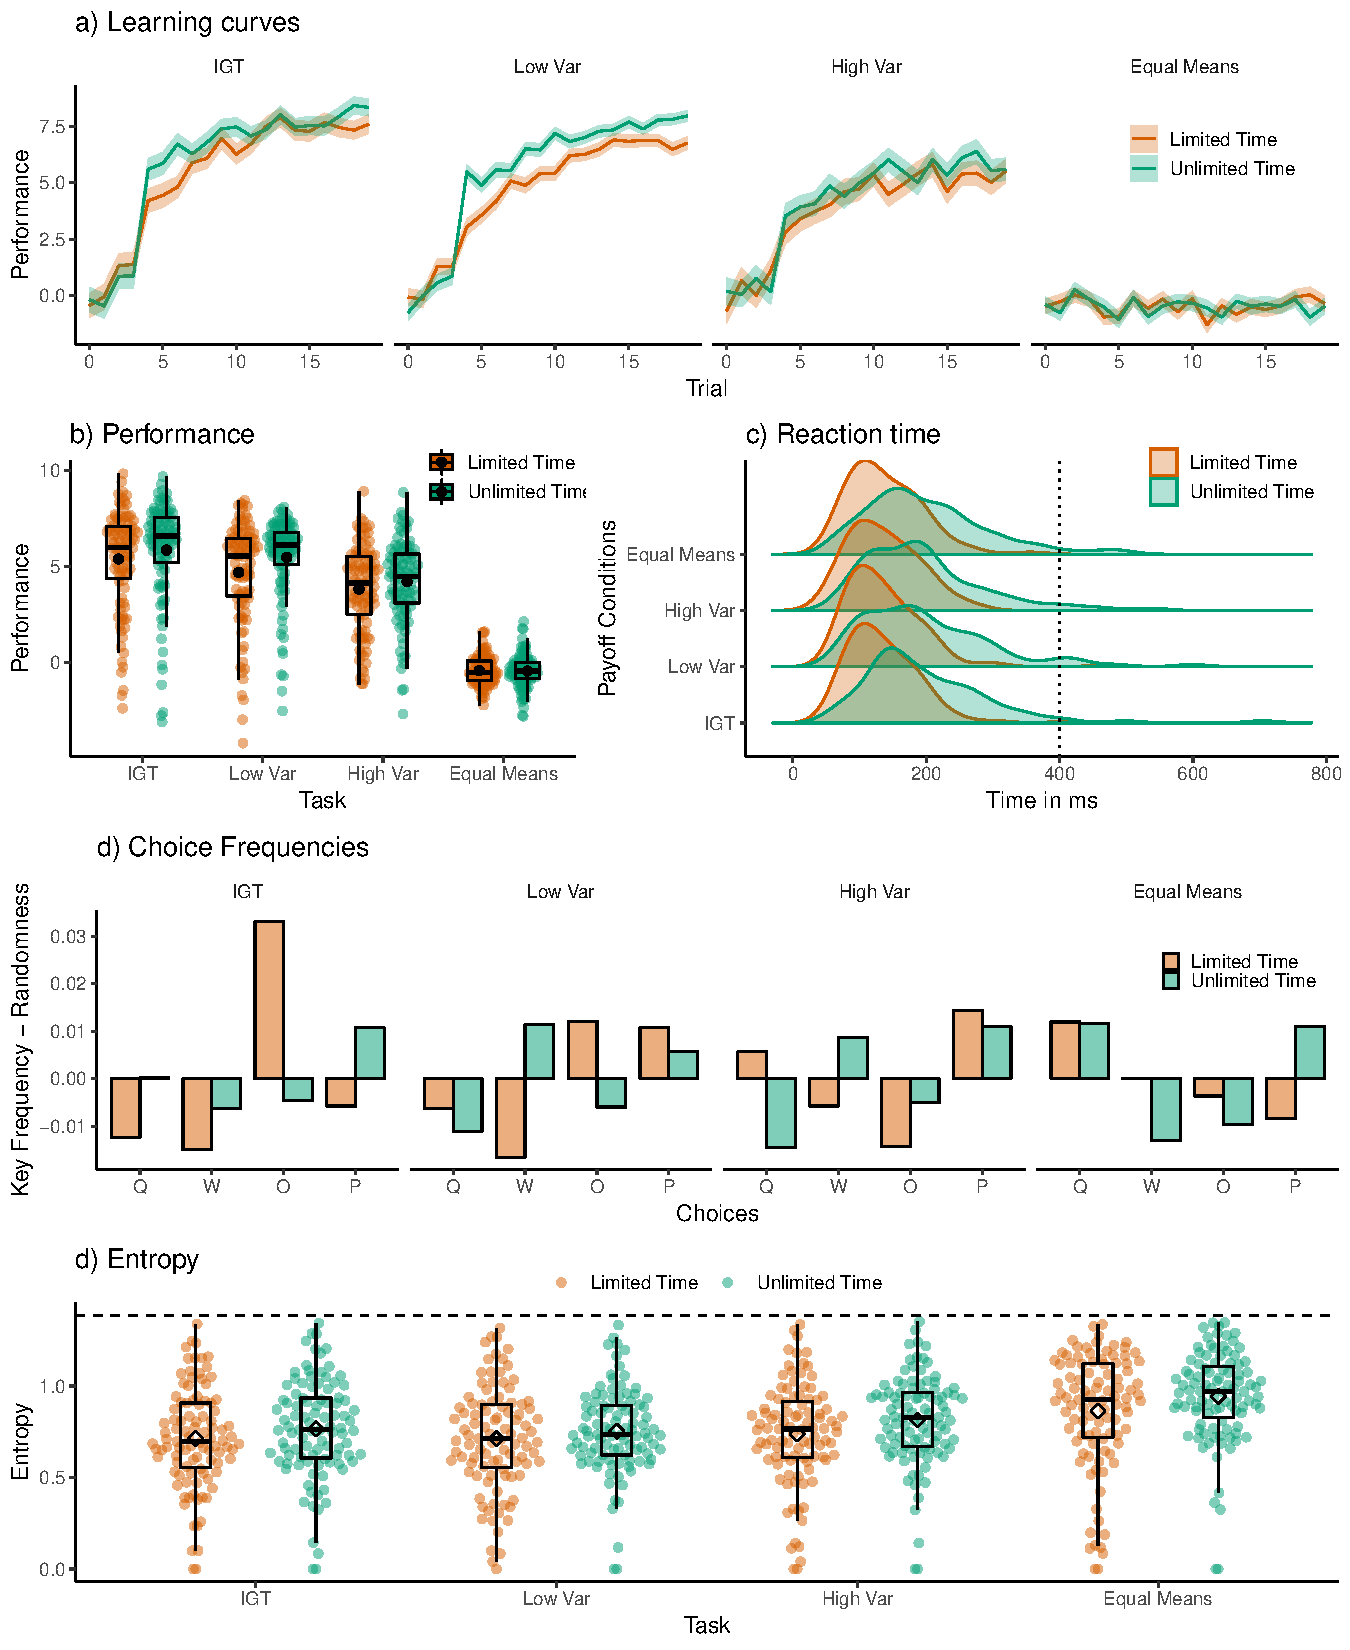
\includegraphics[width=1\textwidth]{Plots/Behaviorplots.pdf}
    \caption[Behavior Analysis Plots]{\textbf{a)} Learning curves. The learning curves over the four payoff conditions and the time conditions were created by calculating the mean reward on each trial per participant per condition combination. \textbf{b)} Average performance. The average performance for each participant over the condition combination. \textbf{c)} Reaction Time. The reaction time for each condition combination do not vary significantly, however participants are faster in the limited time condition. The dotted line represents the 400ms limit. \textbf{d)} Choice Frequency. The choice frequency shows how likely an option is chosen. \textbf{e)} Entropy. The Entropy stands for the choice diversity. A high entropy is equal to switching between options rather than staying at one option. }
    \label{fig:BehaviorPlots}
\end{figure}
\subsection{Performance}
Participants accumulated worse rewards in the limited time conditions ($t(98)=-3.1$, $p=.003$, $d=0.31$, $BF>100$).
In the payoff conditions, participants performed better in Low Variance conditions than in High Variance condition ($t(98)=6.2$, $p<.001$, $d=0.62$, $BF>100$). However, participants performed better in High Variance conditions than in the Spaced Means condition ($t(98)=25.5$, $p<0.001$,$d=2.6$,$BF>100$). The IGT performed the best and so better than the Low Variance condition ($t(98)=3.2$, $p=.002$, $d=0.33$, $BF=14.3$).

\subsection{Reaction Time}
On average participants decide within $186 ms$, they were faster in limited time conditions than unlimited time conditions ($t(98)=-9.7$, $p<.001$, $d=0.98$, $BF>100$). 

\subsection{Choice Frequencies}
Choice frequencies are the probabilities for choosing the different arms. We subtracted a randomness probability of $0.25$ of each arm, which is the probability of choosing an arm by chance. 
Under time pressure, participants preferred to chose low variance option (O for IGT; Q for Equal Means) over high variance option (P for IGT and Equal means) in the IGT and Equal means conditions. This indicates that under time pressure, participants are risk-averse, while under unlimited time participants were more risky by taking the high variance options.
Choice frequency dropped after the fifth trial. 

\subsection{Entropy}
We calculated the Shannon entropy of each round, which gives us a choice distribution over the four arms.
This means it shows us the average information gain when an arm is played: if the entropy is high then the information content we receive is also high and the current information we have is low. If the entropy is low, then we do not gain much information, this means we can easily predict the outcome.The maximum entropy  of 1 is reached when each option is played five times, because this will give us the most information about all options. The entropy is low when only one option is chosen for all the trials, because then we do not get any new information content.
Accordingly, if the entropy is high, then there is a higher diversity in the participants' choices.

We found a higher entropy for the unlimited time condition ($t(98)=5.8$, $p<.001$, $d=0.58$, $BF>100$). This shows a preference for more diversity during unlimited time rounds, which suggests a higher exploration during those rounds. However, under the low var condition, participants had a higher entropy in unlimited time rounds but this was not significant ($t(98)=2.4$, $p=.0.2$, $d=0.23$, $BF=1.6$).
%Not sure what to do with it:if we should leave it in or not.
Considering only the payoff conditions, participants had a higher entropy in the equal means condition than in any other payoff condition. This is supported by the repetition of choosing the same option again, which is the lowest of all payoff conditions. 
Furthermore, the repetition of the same option is higher in limited time rounds than unlimited time rounds over all 20 trials ($t(7919)=20.2$, $p<0.01$, $d=0.23$, $BF>100$). 

\section{Discussion}
The current behavioral results suggest that time pressure has an effect on the uncertainty bonus that is associated with directed exploration. The uncertainty bonus directs the agent that has to chose, to more uncertain options. Thus these options gain a bonus. 

When we take a look at the choice frequencies of the different arms of the IGT condition, we see that during limited time condition, participants rather chose arms with a high mean but a low uncertainty, while they do not show this behavior in unlimited time conditions, rather the opposite; there was a tendency to chose the high mean and high variance arm more often. 

The entropy, or rather the choice diversity is also an indicator of this rejection of an uncertainty bonus: Unlimited time conditions have a higher diversity than limited time conditions. This means that under unlimited time, participants change the key they are pressing more often, while they rather stay at the same key under time pressure.  

Until now, we have seen the influence of time pressure on the behavioral level, however, we cannot access the influence on a process level from only considering the behavioral data. In order to understand the influence on uncertainty and the exploration bonus in exploration-exploitation task, we have to take the analysis a step further: with modeling human behavior. 
